\documentclass{standalone}

\usepackage{tikz}
\usetikzlibrary{arrows, arrows.meta, calc, shapes}
\usepackage{datastore}

\begin{document}

\tikzset{>={Latex[length=3mm,width=2mm]}}
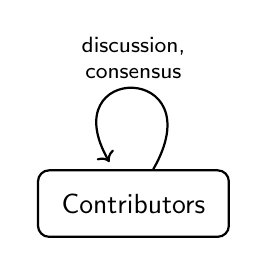
\begin{tikzpicture}[
  font=\sffamily,
  every matrix/.style={ampersand replacement=\&, column sep=4cm, row sep=4cm},
  interface/.style={draw, thick, regular polygon, regular polygon sides=4, inner sep=0},
  process/.style={draw, thick, rounded corners, inner sep=.3 cm},
  datastore/.style={draw, thick, shape=datastore, inner sep=.3cm},
  to/.style={->, shorten >=3pt, thick, font=\sffamily\footnotesize},
  both/.style={<->, shorten >=3pt, thick, font=\sffamily\footnotesize},
  every node/.style={align=center}]

  % Position the nodes using a matrix layout
  \matrix{
    \node[process] (editor) {Contributors}; \\
  };

  % Draw the arrows between the nodes and label them.
% \draw[to] (content) to[bend left=25] node[midway, right] {articles, \\ edits} (ai);
% \draw[to] (ai) to[bend left=25] node[midway, below] {raw scores} (scores);
% \draw[to] (scores) to[bend left=25] node[midway, left] {scores, \\ context} (editor);
% \draw[to] (scores) to[bend right=25] node[midway, left] {scores, \\ context, \\ justifications} (patroller);

  % edits: Two-way cycle with label between legs.
% \draw[to] (editor) to[bend left=25] (content);
% \draw[to] (content) to[bend left=25] (editor);
% \node [align=flush center] at ($(editor)!0.5!(content)$) {edits, \\ curation};

  % judgments: Two-way cycle with label between legs.
% \draw[to] (patroller) to[bend left=25] (judgments);
% \draw[to, dashed] (judgments) to[bend left=25] (patroller);
% \node [align=flush center] at ($(patroller)!0.5!(judgments)$) {judgments, \\ rationales};

% \draw[to] (judgments) to[bend right=25] node[midway, right] {false positives, \\ training data} (ai);
  
  \draw[to] (editor) to[loop, out=60, in=120, looseness=8] node[midway, above] {discussion, \\ consensus} (editor);

% \draw[to, dashed] (patroller) to[loop, out=-60, in=-120, looseness=5] node[near end, left] {discussion, \\ consensus} (patroller);

\end{tikzpicture}

\end{document}
